%\subsection{Estimating Bathymetry}

In this Section, we describe some experimental results with simulated and real data using few existing nonlinear optimization tools that we used in our preliminarily experiments (see Section \ref{inv_techniques}). Note that our forward model is nonlinear as described in Section \ref{forwardproblem} and it can not be written as a matrix equation system. Therefore, in this Bathymetry inversion, we can not use any inverting method where it needs forward operator as a explicit matrix operator (e.g., \verb|tikhonov| and  \verb|lsqnonneg|     
 Matlab\textsuperscript{\textregistered} functions need forward operator as a matrix). Moreover, the bounds of the true Bathymetry in the interested near shore region is known to be $[0m, 11m]$. Therefore, we picked the inverse solvers that enable us to incorporate that prior knowledge too. 

\subsection{Simulated Data}
In this study, Gaussian noise corrupted simulated wave numbers (see Section \ref{inv_techniques} for more details) are generated by 
\begin{equation}
\mathbf{k}_s = A(\mathbf{h}_t) + \mathcal{N}(0, \nu^2),
\end{equation}
where $A(\cdot)$ represents the nonlinear forward operator defined in Section \ref{forwardproblem}, $\mathbf{h}_t \in \mathbb{R}_+^n$ is the true Bathymetry vector, and $\mathcal{N}(0, \nu^2)$ is a additive Gaussian noise vector with standard deviation $\nu$, generated in the Matlab\textsuperscript{\textregistered} by $\nu \cdot $\verb| randn(n,1)|. we manufactured wave numbers $\mathbf{k}_s$ for two different grid resolutions, i.e., 10m and 25m (see \ref{Simulated25m} and Fig. \ref{Simulated10m} respectively), to test and tune our inverse methods before working with actual measurements. 



\begin{figure}[H]
\center
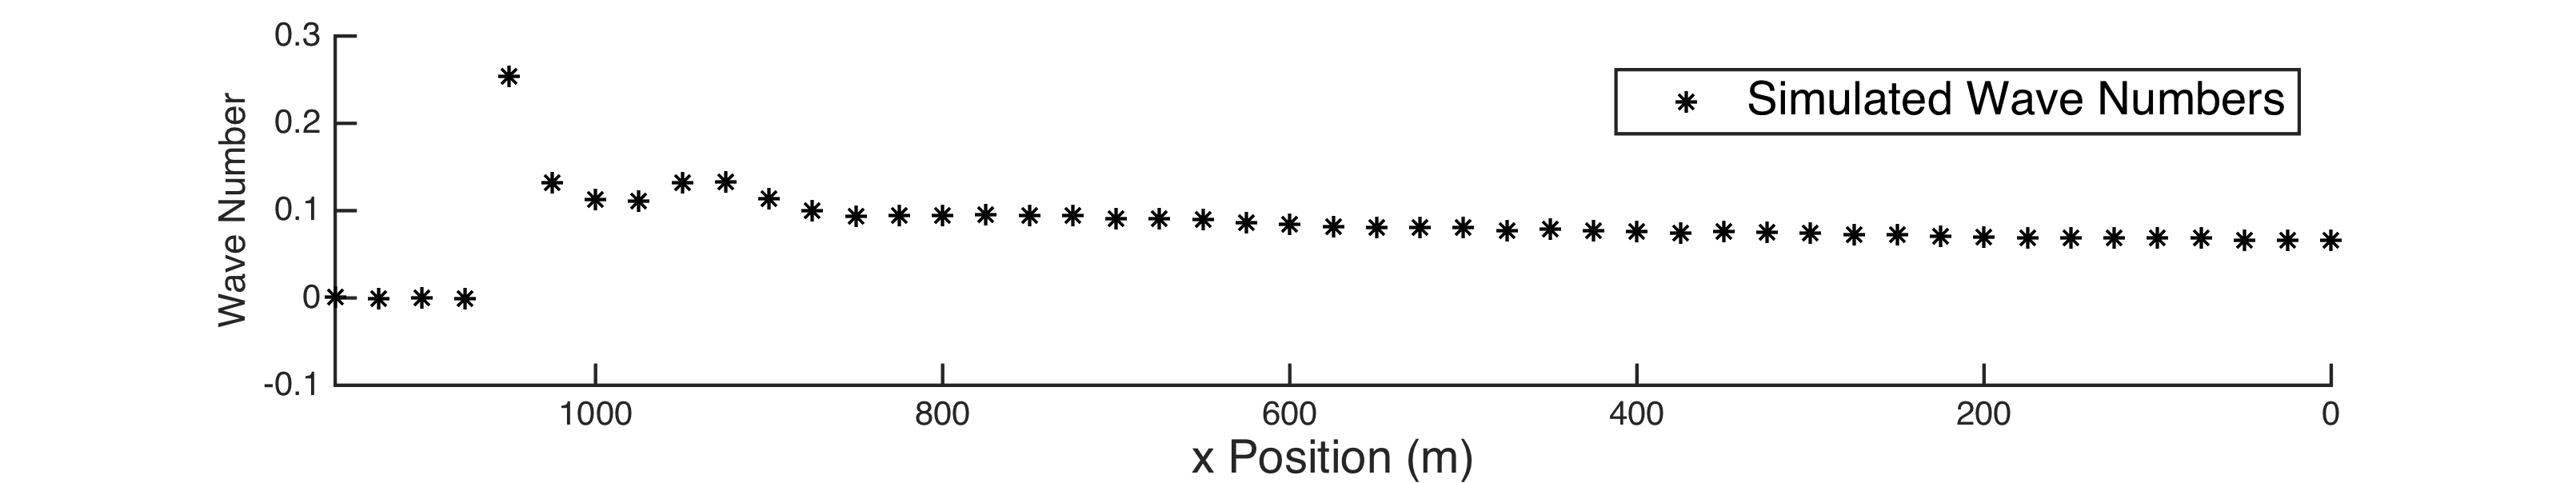
\includegraphics[scale=0.6]{img/simulated_data_k25m.png} 
\caption{1\% noisy ($\nu = 10^{-3}$) simulated wave numbers $(\mathbf{k}_s)$ with 25m grid resolution. Noise (\%) = $\|A(\mathbf{h}_t) -  \mathbf{k}_s\| / \|  \mathbf{k}_s \| \cdot 100$.}
\label{Simulated25m}
\end{figure}

\begin{figure}[H]
\center
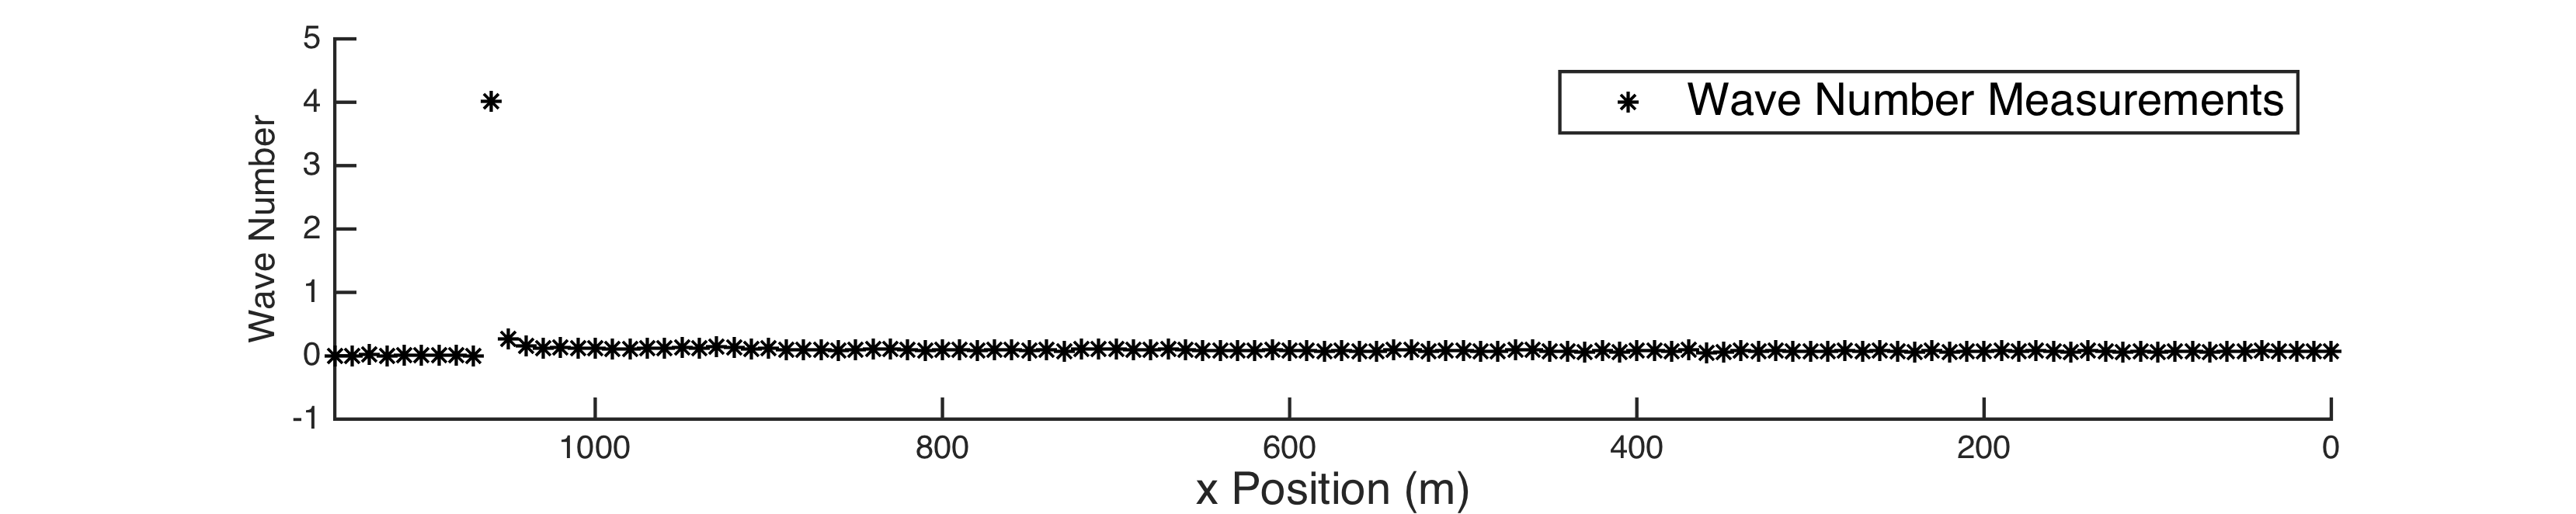
\includegraphics[scale=0.6]{img/simulated_data_k10m.png} 
\caption{2.5\% ($\nu = 10^{-2}$) noisy simulated wave numbers $(\mathbf{k}_s)$ with 10m grid resolution. Noise (\%) = $\|A(\mathbf{h}_t) -  \mathbf{k}_s\| / \|  \mathbf{k}_s \| \cdot 100$. }
\label{Simulated10m}
\end{figure}


\subsection{Real Data}\label{realData}

As discussed in Section \ref{datak}, measured wave numbers, $\mathbf{k}_m$, are provided by the USACE for the month of October 2015 at half hour increments during day light hours. To test our inversion schemes, we choose a wave number profile based off of two constraints; available bathymetry data near the time of the chosen profile and minimal noise in the measured data, which is associated with calmer ocean conditions. According to these constraints, we focus on wave number measured around October 9th as the conditions were relatively calm and a survey executed near that time. Figure \ref{RealData_oct09} shows measured profiles for October 9th, 2015 12:00:00 - 23:00:00 (UTC). It should be noted that multiple wave numbers were provided by the USACE at each measurement location; the dominant wave number were considered in this project. Also note that the measured wave numbers near the shore (x Position $>$ 1050m) and the deep end (x Position $<$ 350m) are not available.


\begin{figure}[H]
\center
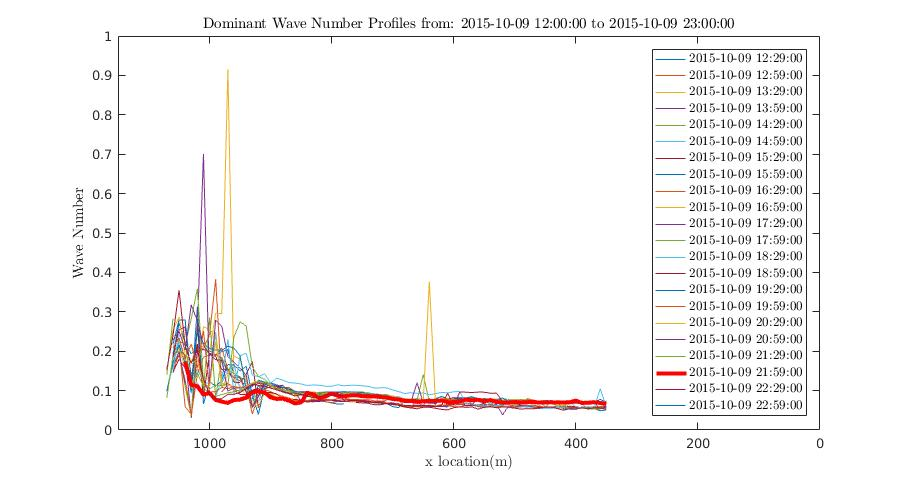
\includegraphics[scale=0.5]{img/Real_k_data.jpg} 
\caption{Real measurements of wave numbers $(k)$ on the 09th October 2015.}
\label{RealData_oct09}
\end{figure}

Upon inspection of each wave number profile from this time period, it is evident that the profile corresponding to 21:59:00 UTC (highlighted in red) contains little noise relative to the others; this profile will be used for our inversion schemes.


\subsection{Ordinary Least-Squares Fitting Results} \label{OrdLstSqrRes}
Here, we approximate the unknown bathymetry by solving the following optimization problem:
\begin{equation}\label{LS-BC}
\mathbf{\hat{h}}= \underset{\mathbf{0} \preceq \mathbf{h} \preceq \mathbf{11} }{\arg \min} \ \  \|  A(\mathbf{h}) -  \mathbf{k} \|_2^2.
\end{equation}
%<<<<<<< HEAD
In particular, we modify the ordinary least squares problem in \eqref{LS} to a bounded constrained optimization problem to incorporate the known bathymetry bounds. Based on the preliminary studies and referring the Matlab\textsuperscript{\textregistered} documentation, we decided to use the Matlab's \verb|lsqnonlin| function to solve this problem \eqref{LS-BC} for the simulated and real $\mathbf{k}$ measurements. According to the Matlab\textsuperscript{\textregistered} documentation, here we have two algorithm choices: \textit{trust-region-reflective} (default) or \textit{Levenberg-Marquardt}. However, the Levenberg-Marquardt algorithm does not handle bound constraints. Therefore, we use the trust-region-reflective algorithm (See \cite{trustregion} for more details regarding the algorithm) inside the \verb|lsqnonlin| function to recover the unknown depth parameter. Rather than input the sum of squares of the objective function in \eqref{LS-BC} to the \verb|lsqnonlin| function, it requires a user-defined vector-valued function $f(\mathbf{h}) = A(\mathbf{h}) -  \mathbf{k}$ as the function argument along on the boundary conditions. 
%=======
%In particular, here we modify the ordinary least squares problem in \eqref{LS} to a bounded constrained optimization problem to incorporate the known bathymetry bounds. Based on the preliminary studies and referring the Matlab documentation, we decided to use the Matlab's \verb|lsqnonlin| function to solve this problem \eqref{LS-BC} for the simulated and real $\mathbf{k}$ measurements. According to the Matlab documentation, here we have two algorithm choices: \textit{trust-region-reflective} (default) or \textit{Levenberg-Marquardt}. However, the Levenberg-Marquardt algorithm does not handle bounded constraints. Therefore, we use the trust-region-reflective algorithm (See \cite{trustregion} for more details regarding the algorithm) inside the \verb|lsqnonlin| function to recover the unknown depth parameter. Rather than input the sum of squares of the objective function in \eqref{LS-BC} to the \verb|lsqnonlin| function, it requires a user-defined vector-valued function $f(\mathbf{h}) = A(\mathbf{h}) -  \mathbf{k}$ as the function argument along on the boundary conditions. 
%>>>>>>> 1f18d0b22683c8c5406c9d75230a94687fa68929

\begin{figure}[H]
\center
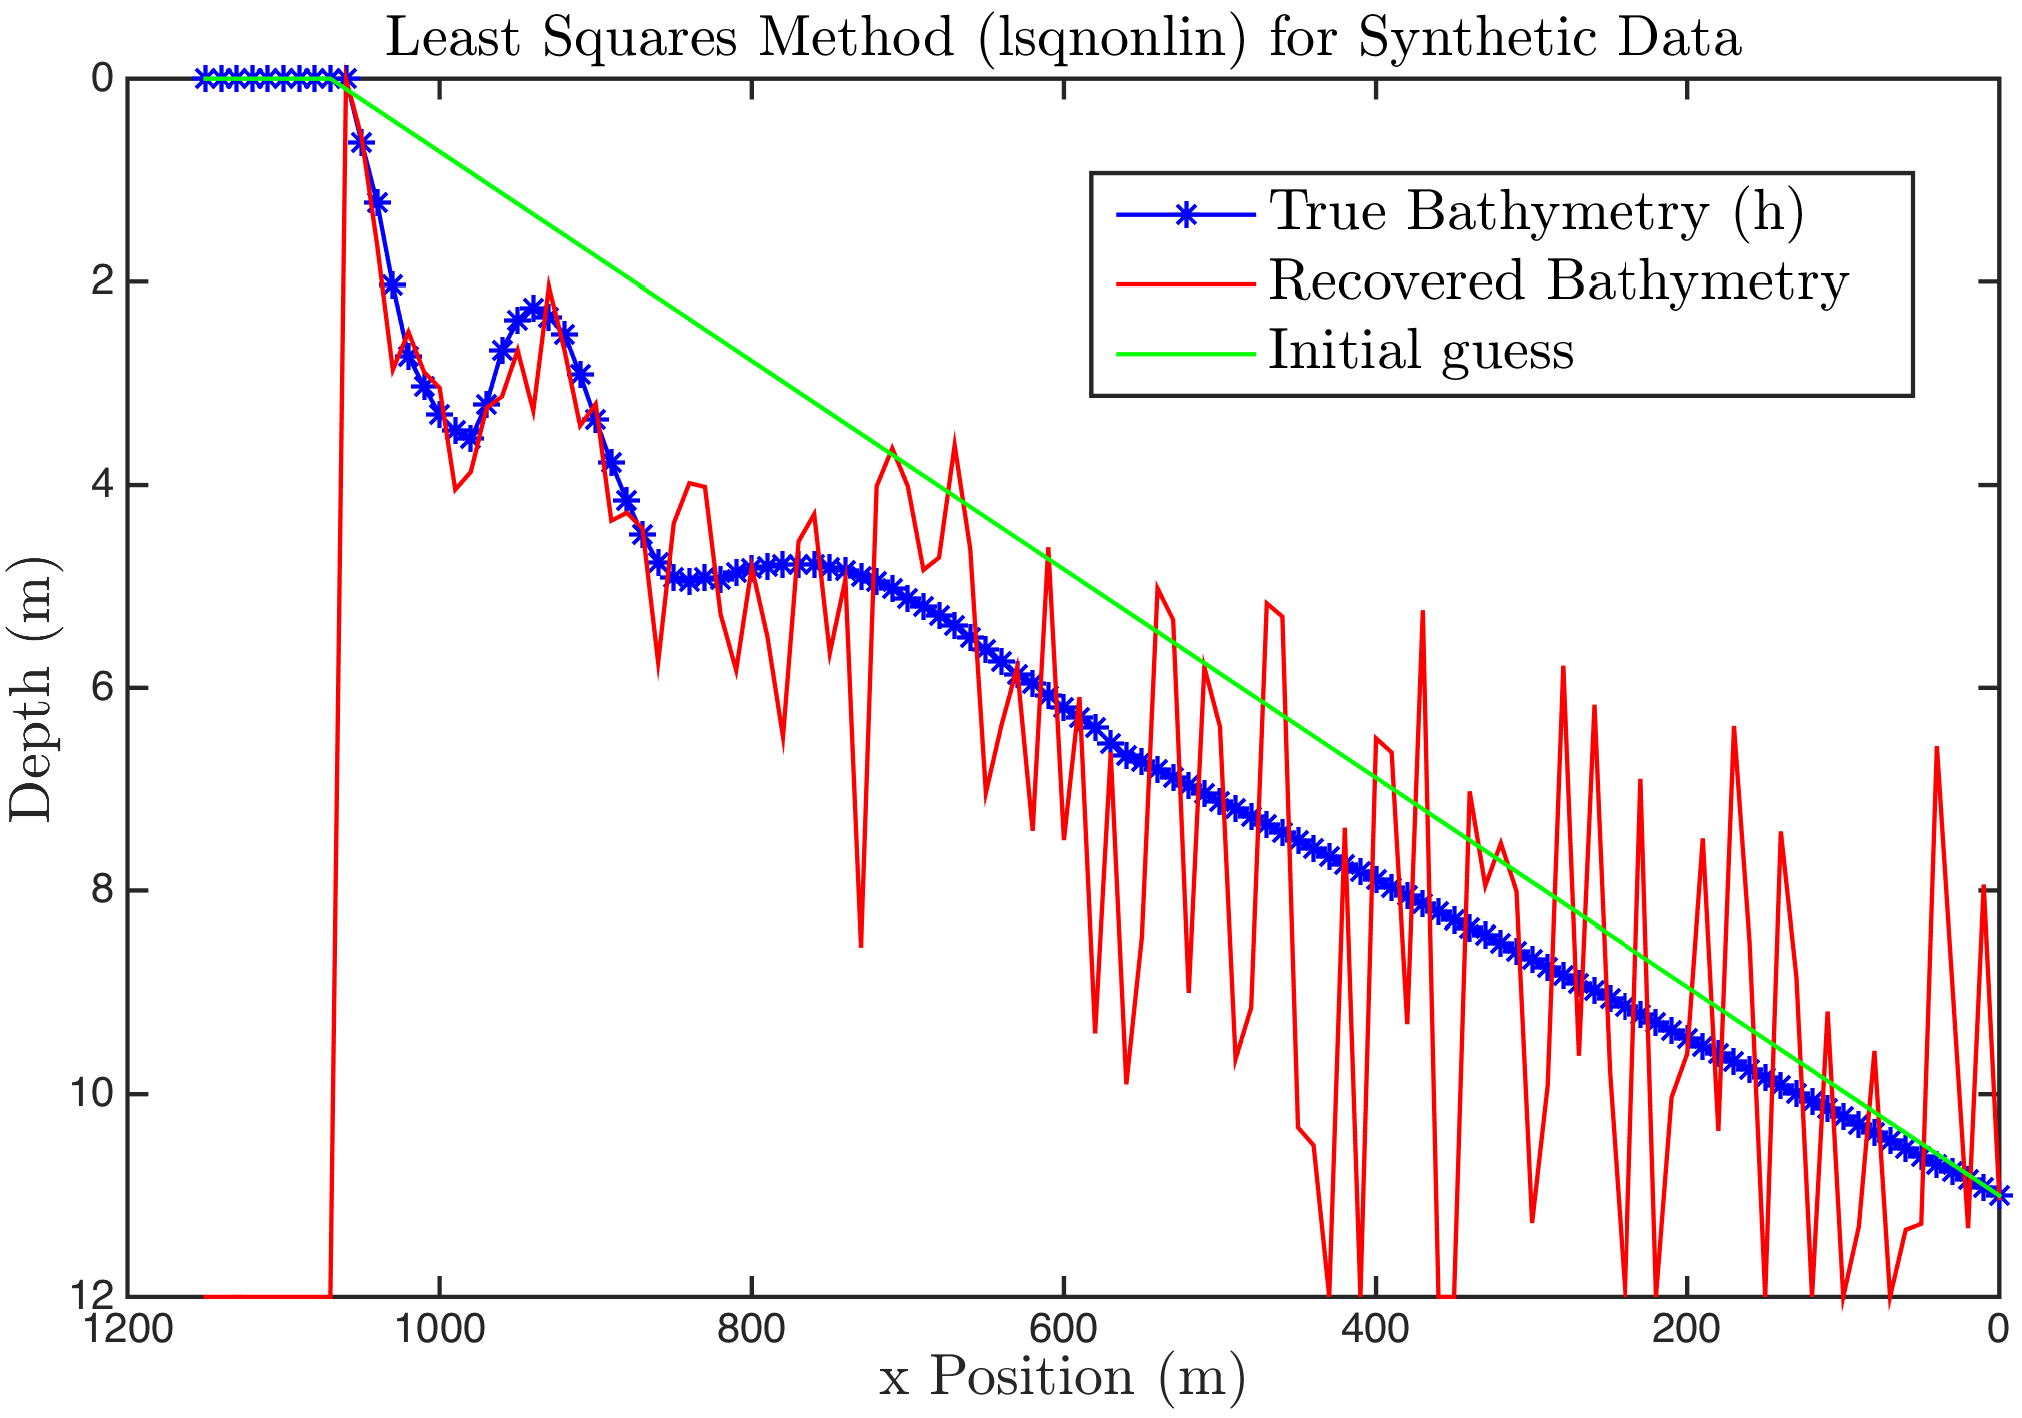
\includegraphics[scale=0.6]{img/lsqnonlin_simulated_10m.png} %plot20 
\caption{Ordinary least-squares reconstruction of depth $\mathbf{h}$ using the simulated data.}
\label{lsqnonlin_simulated}
\end{figure}
First, we run the \verb|lsqnonlin| function on the synthetic data $\mathbf{k}_s$ with 10m grid resolution. The least-squares method captured the most interesting and important sand bar near the shoreline (see Fig. \ref{lsqnonlin_simulated} from 800m to 1000m area). However, the recovered depth is unstable from 600m to the deep-end due to the ill-conditioned nature of the nonlinear forward operator. 

%Note that a linear function is used as the initial guess for this numerical method  and which is represented in a green color line. 
\begin{figure}[H]
\center
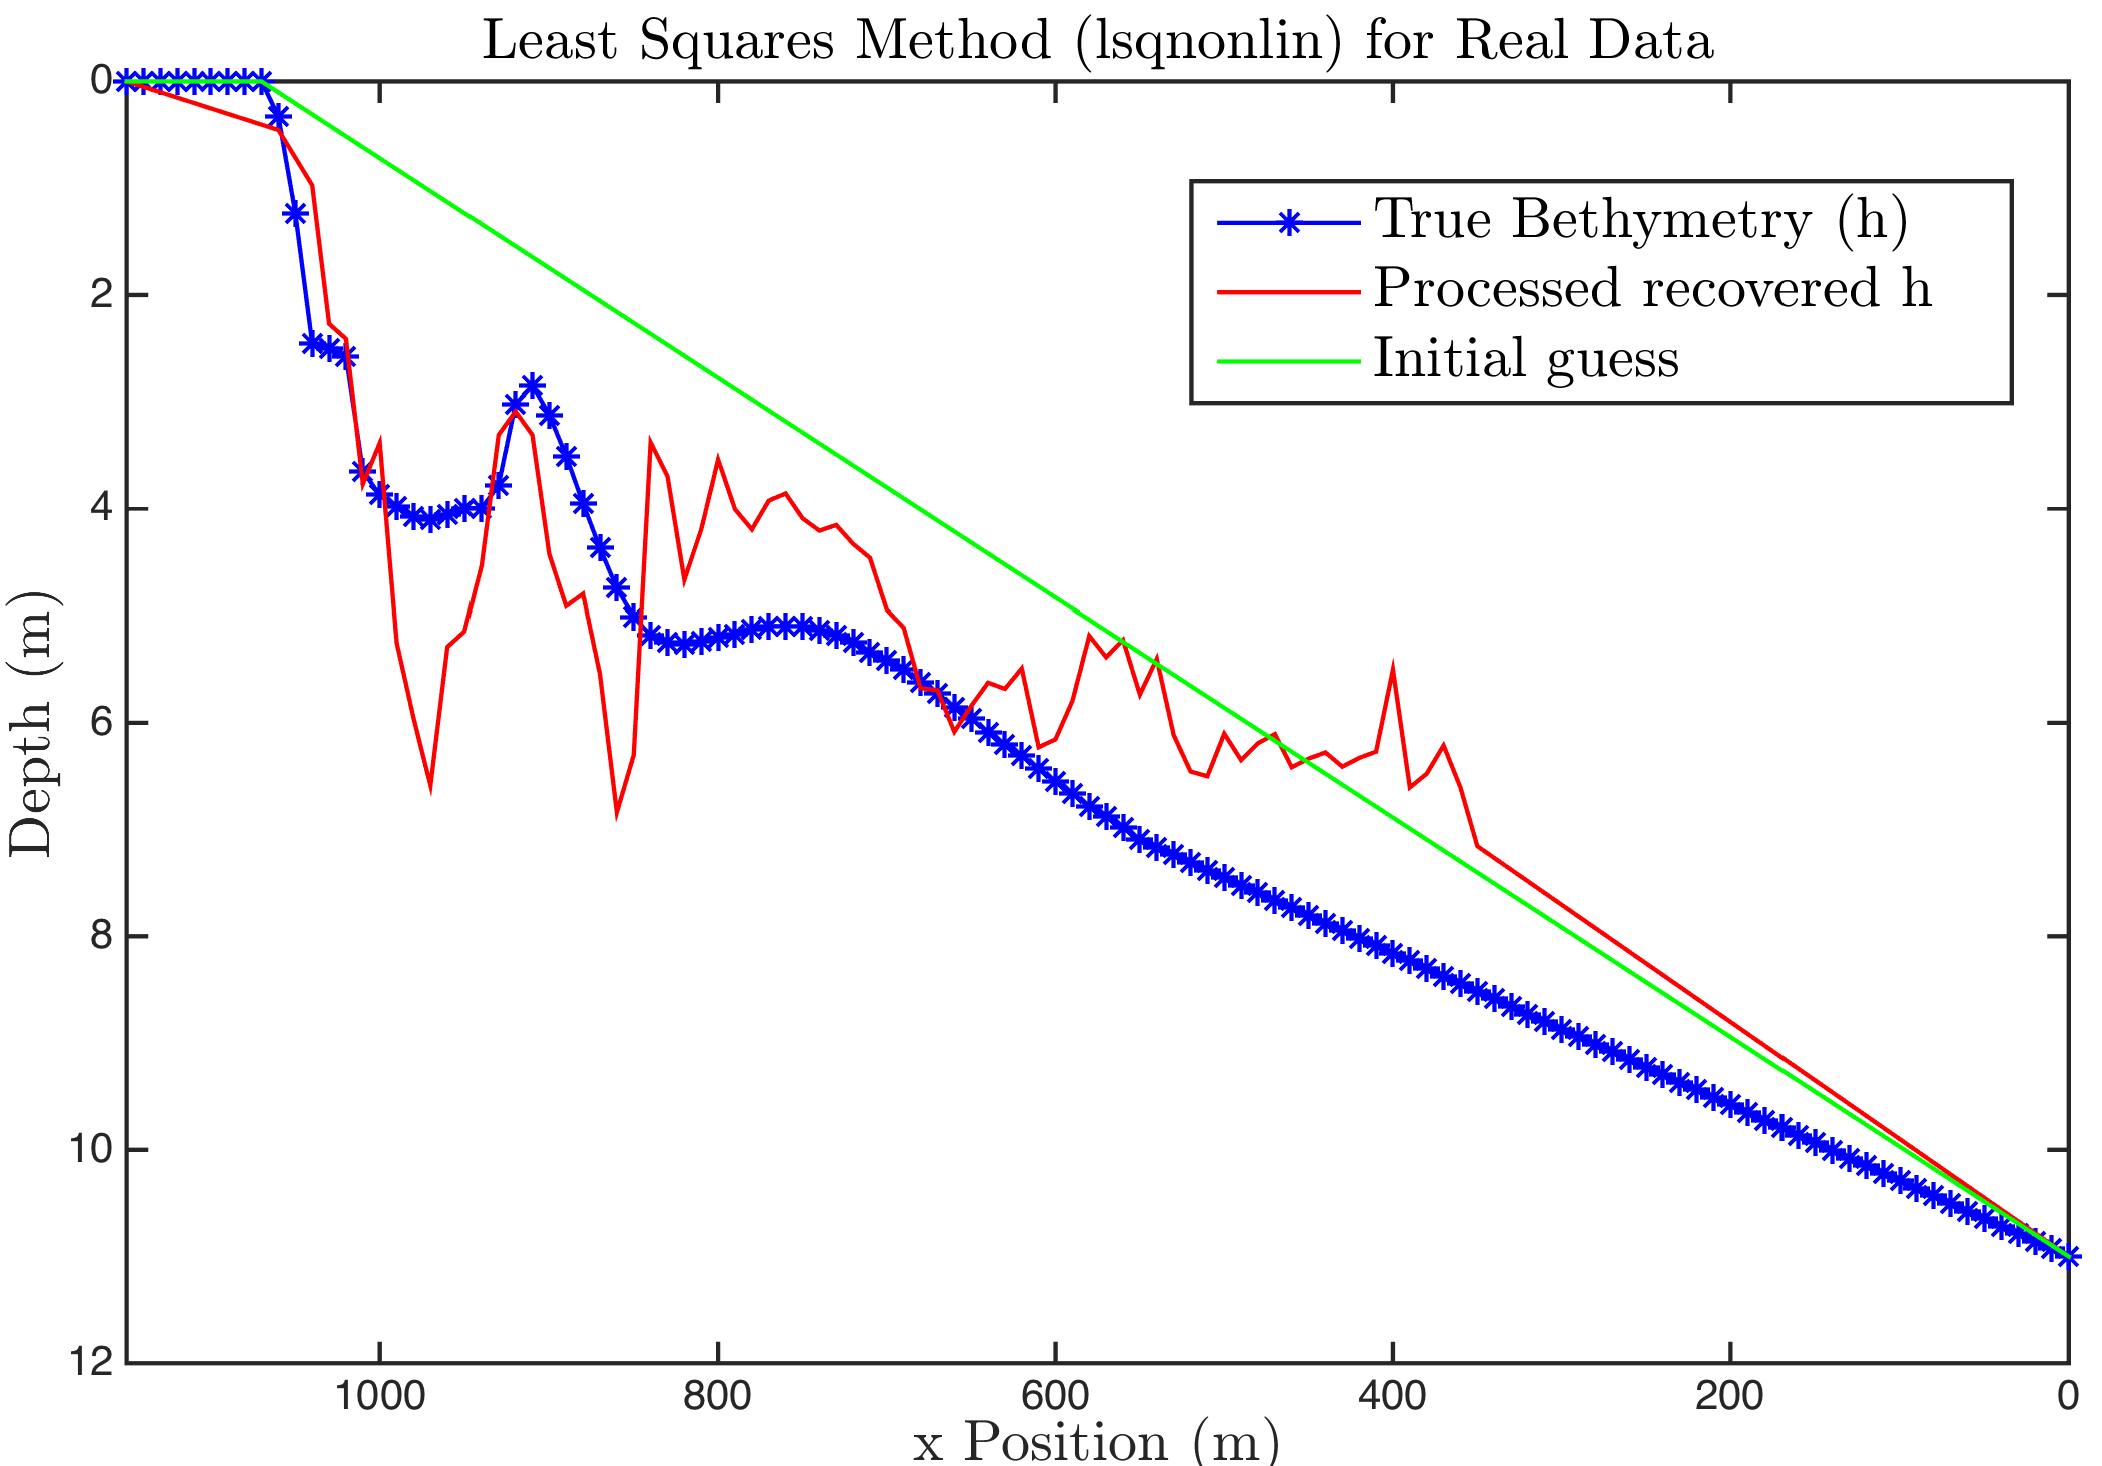
\includegraphics[scale=0.6]{img/lsqnonlin_real_data_oct09.png} %plot20 
\caption{Ordinary least-squares reconstruction of the depth $\mathbf{h}$ using the real data.}
\label{lsqnonlin_real}
\end{figure}

After considering the synthetic data, the real wave number measurements $\mathbf{k}_m$ discussed in Section \ref{realData} are used with the same Matlab's \verb|lsqnonlin| optimizer. In this reconstruction, we capture the near-shore topography including the sand bar with $53\%$ root mean square error (see Fig. \ref{lsqnonlin_real}); errors sea-ward of the sand bar are again attributed to the ill-conditioned nature of this problem in combination with noise in the measured wave number. It should be noted that we have interpolated and processed the depth reconstruction based on the missing measurement locations. 


\subsection{Tikhonov Regularized Results} \label{TickReg}

In order to get more stable solution than the ordinary least squares solution in Fig. \ref{lsqnonlin_simulated}, we decided to solve the following bounded-constrained Tikhonov regularization optimization problem:
\begin{equation}\label{LS-regBC}
\mathbf{\hat{h}} = \underset{\mathbf{0} \preceq \mathbf{h} \preceq \mathbf{11}}{\arg \min} \ \ \|  A(\mathbf{h}) -  \mathbf{k} \|_2^2  +   \| \boldsymbol{\alpha} \cdot  \mathbf{h}\|_2^2,
\end{equation}
%<<<<<<< HEAD
with the hope of getting more stable solution. Specially, here we use a vector of regularization parameters to balance the trade-off between the data-fidelity and the regularization term according to the x Position. Based on the Matlab's optimization decision table \cite{descTable}, there are only two solvers that we can apply to solve this bounded-smooth-nonlinear problem, i.e., \verb|fmincon| and \verb|fseminf|. In this study, we decided to use  most popular \verb|fmincon| solver, which uses \textit{interior-point} (by default) algorithm internally. According to the Matlab\textsuperscript{\textregistered} documentation, \textit{interior-point} algorithm uses special techniques for large-scale problems and it satisfies bounds at all iterations. 
%=======
%with the hope of getting more stable solution. Specially, here we use a vector of regularization parameters to balance the trade-off between the data-fidelity and the regularization term according to the x Position. Based on the Matlab's optimization decision table []\cite{descTable}, there are only two solvers that we can apply to solve this bounded-smooth-nonlinear problem, i.e., \verb|fmincon| and \verb|fseminf|. In this study, we decided to use  most popular \verb|fmincon| solver, which uses \textit{interior-point} algorithm internally. According to the Matlab documentation, \textit{interior-point} algorithm uses special techniques for large-scale problems and it satisfies bounds at all iterations. 
%>>>>>>> 1f18d0b22683c8c5406c9d75230a94687fa68929

In this experiment, we heuristically tuned the regularization parameters and recovered the bathymetry with only with $15\%$ root mean square error (see Fig. \ref{fmincon_simulated}) for the synthetic measurements with 25m grid resolution. Note that the recovered bathymetry is much stable and has less fluctuations than the ordinary least squares solution in Fig. \ref{lsqnonlin_simulated}.   
 
\begin{figure}[H]
\center
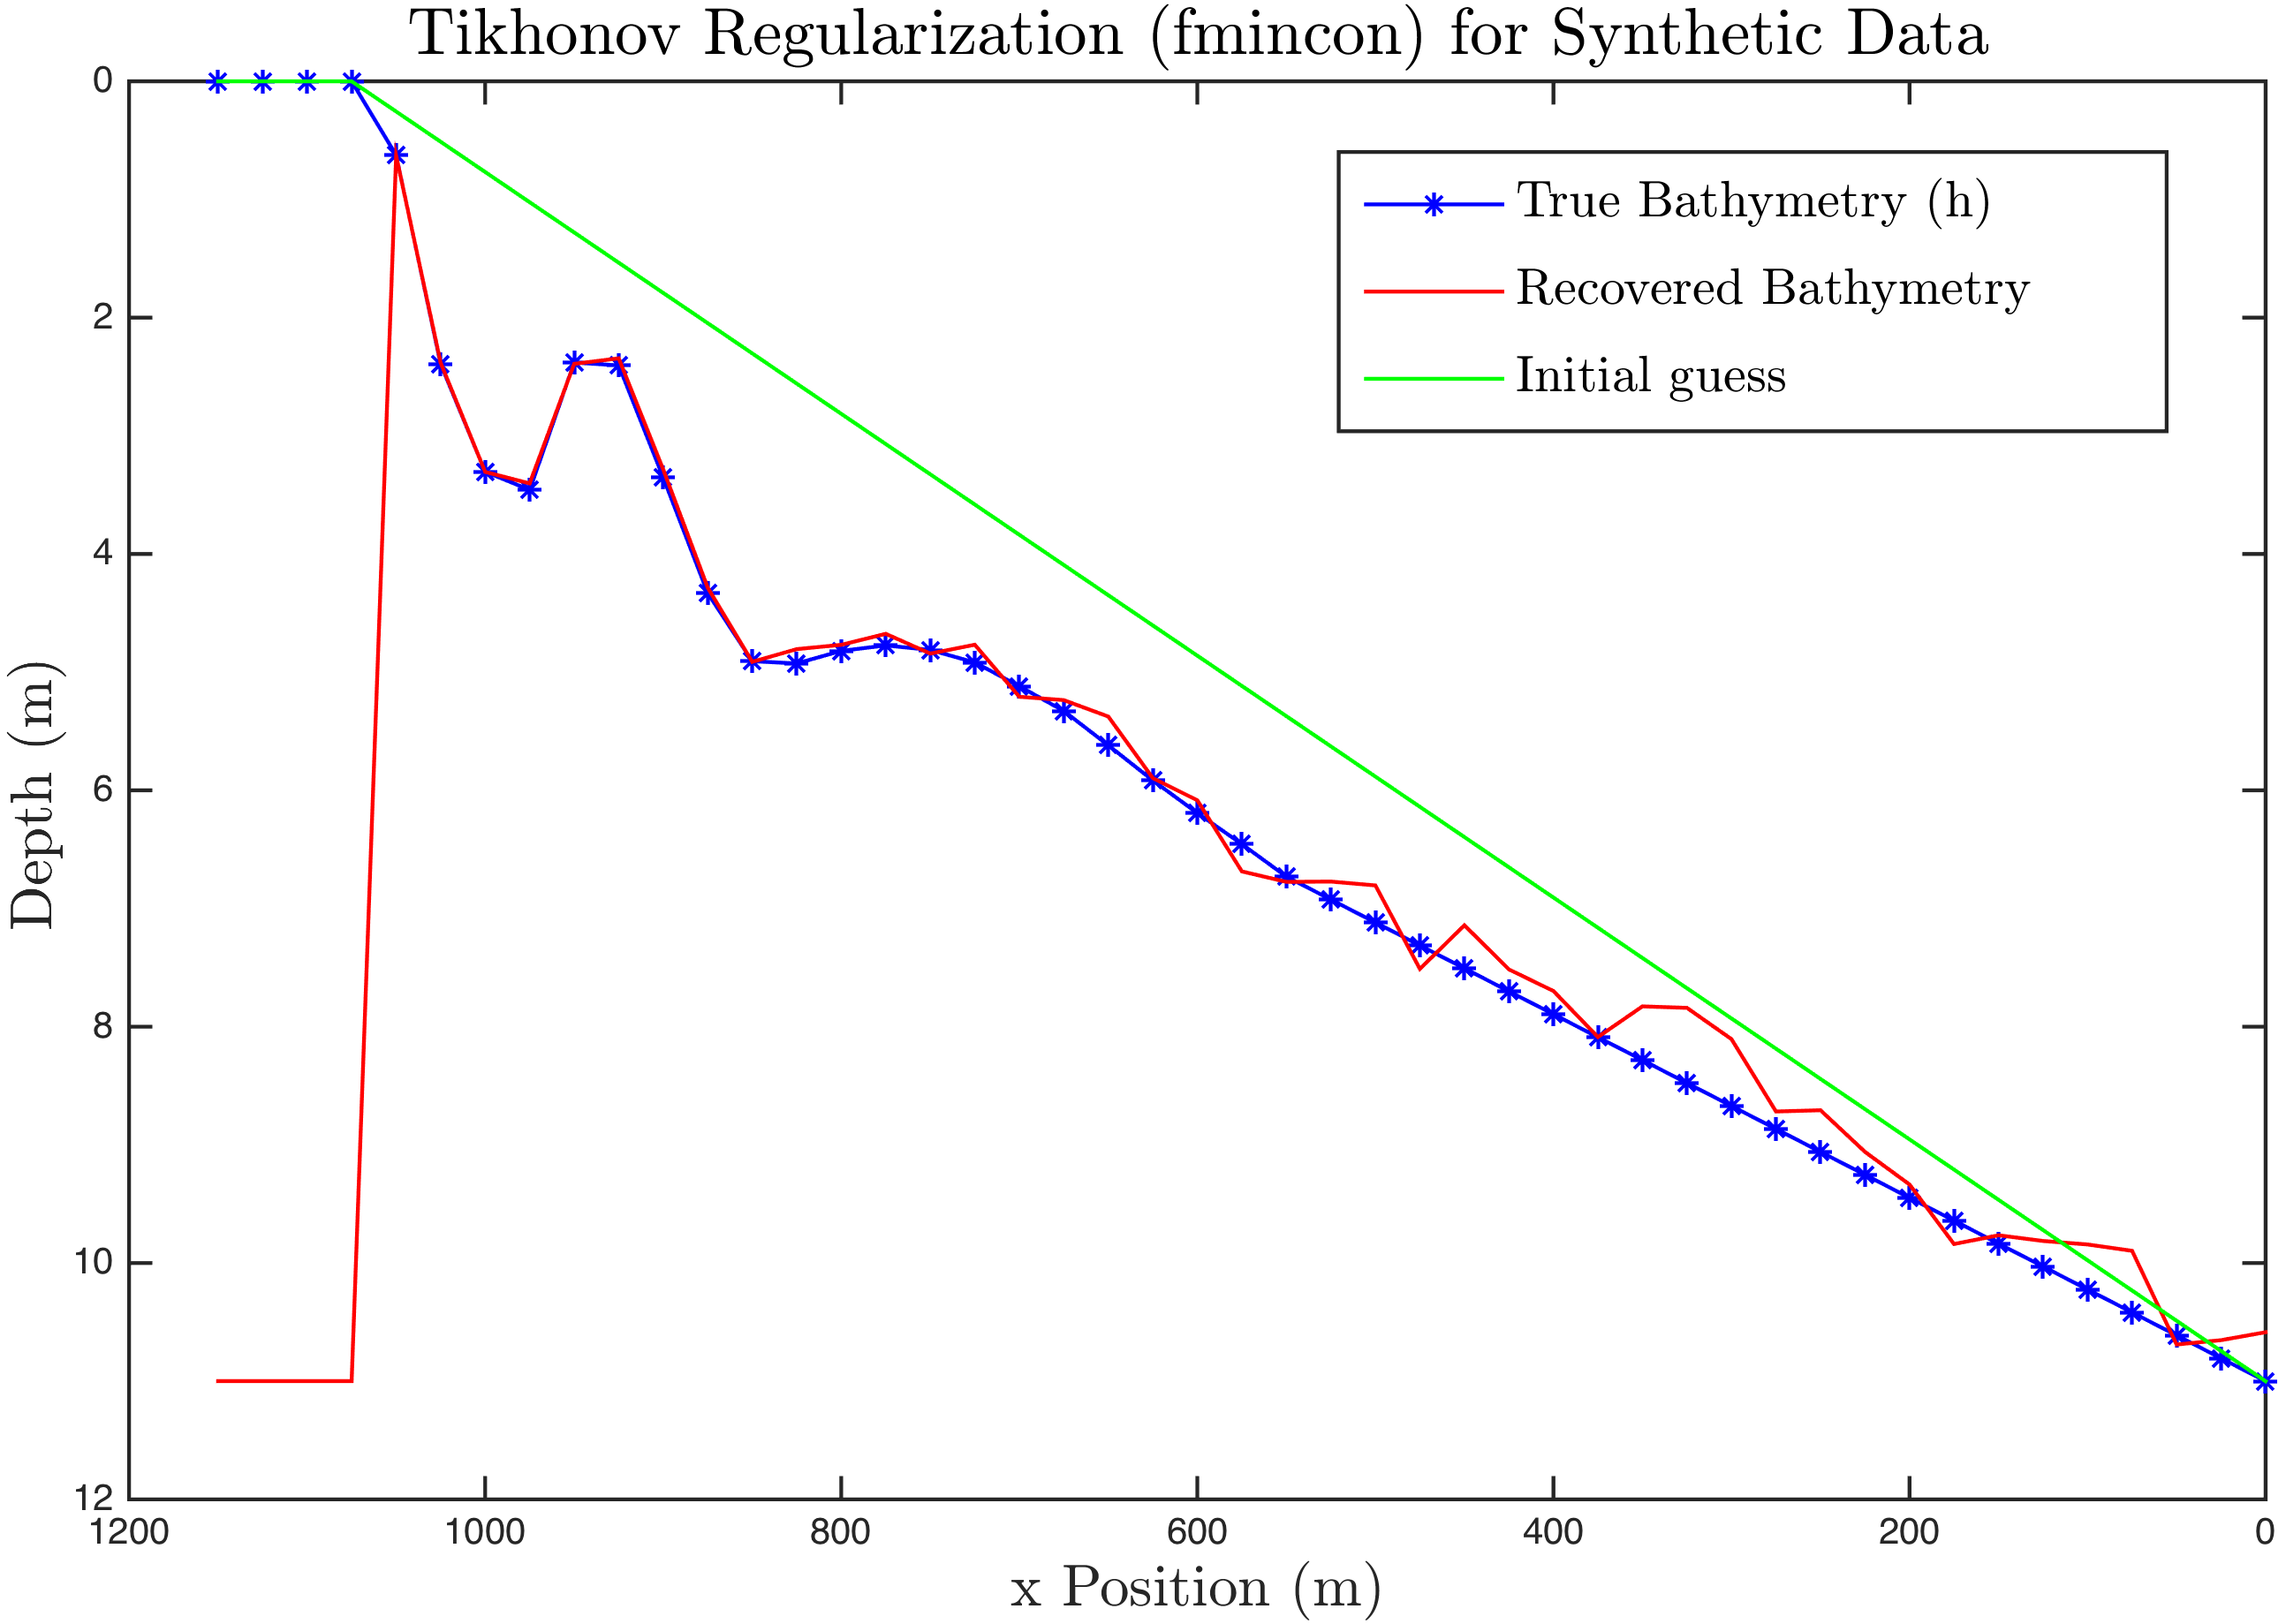
\includegraphics[scale=0.47]{img/fmincon_simulated_25_new.png} %plot20 
\caption{Tikhonov Regularized reconstruction of the depth $\mathbf{h}$ using the simulated data.}
\label{fmincon_simulated}
\end{figure}

Similarly, we run the Matlab's \verb|fmincon| solver to minimize the Tikhonov regularized objective with the real dataset $\mathbf{k}_s$. In this experiment, we were able to recover the sand bar area much accurately with less artifacts (see Fig. \ref{fmincon_real}) but again deviations are noted sea-ward of the sand bar.

\begin{figure}[H]
\center
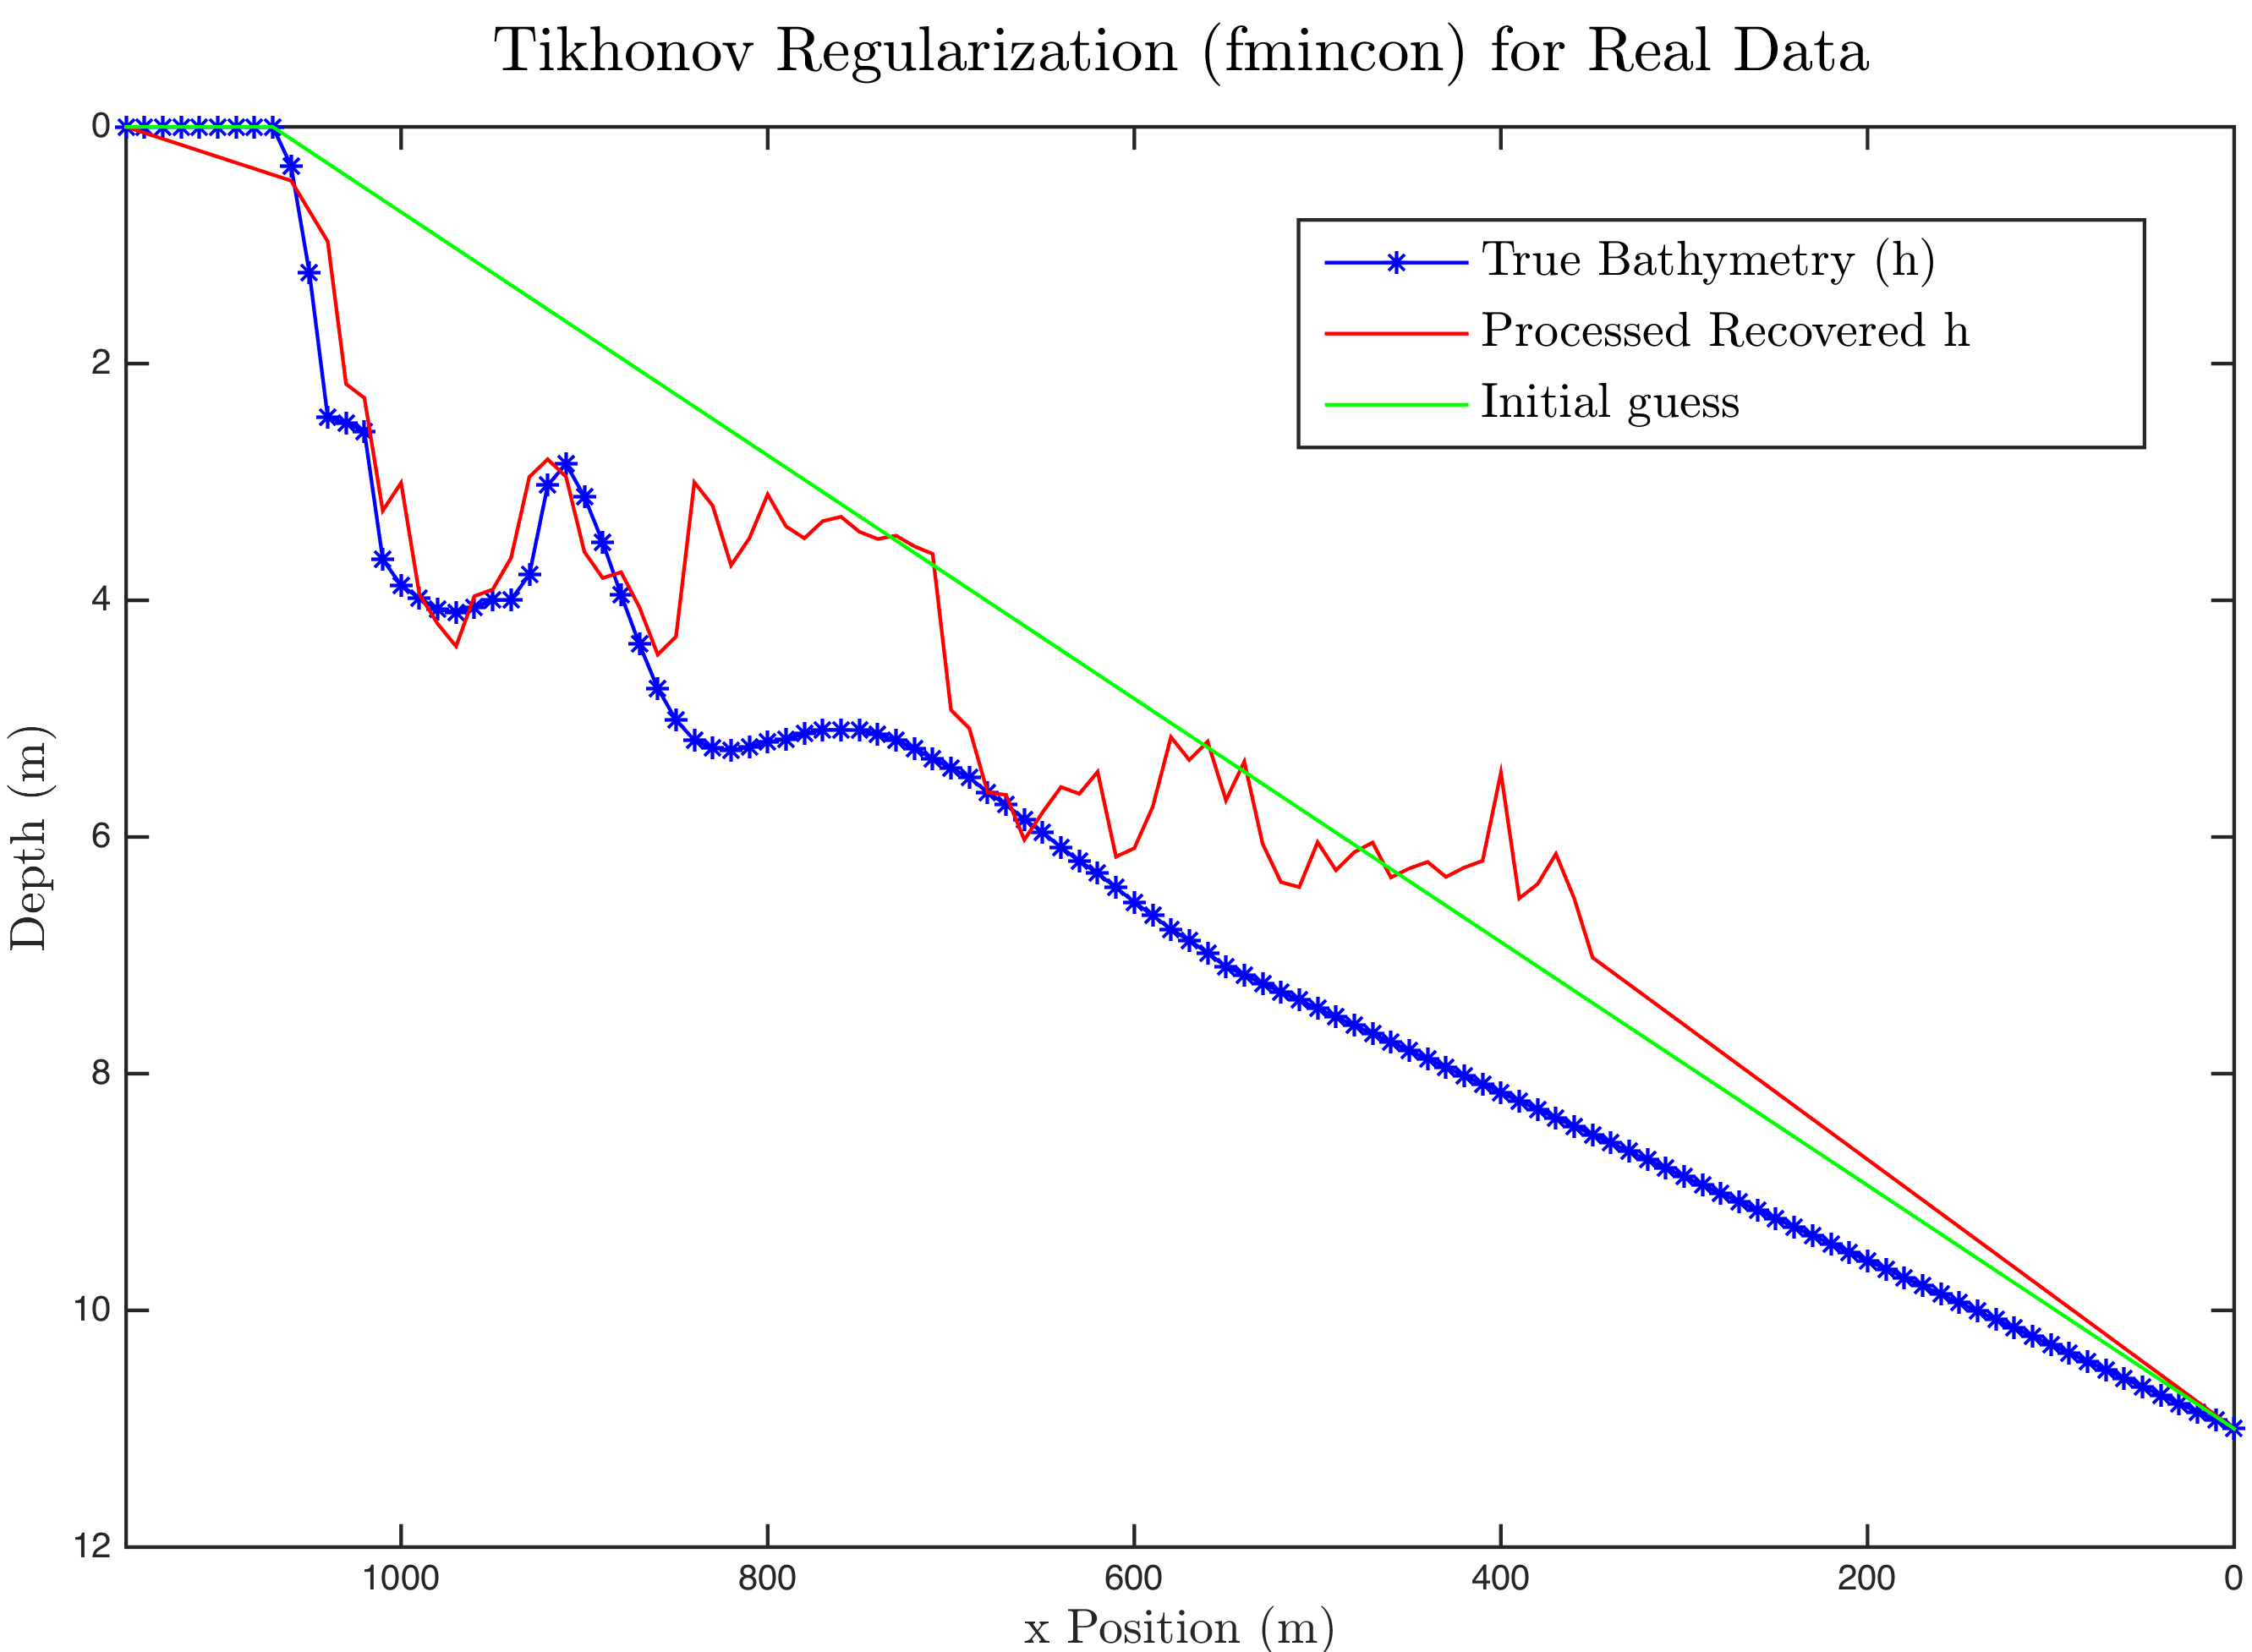
\includegraphics[scale=0.46]{img/fmincon_real_data_oct09.png} %plot20 
\caption{Tikhonov Regularized reconstruction of the depth $\mathbf{h}$ using the real data.}
\label{fmincon_real}
\end{figure}




%\subsection{Bayesian Inference}
%The Bayesian inversion approach samples a posterior distribution of depth profiles. For comparison to the other inversion methods, we consider only the depth at each grid point which corresponds to the maximum of the posterior probability distribution at that point. This is achieved by taking the maximum of the kernel density of the estimated depth distribution at each point along the 1D profile. 
%
%This method is first applied using synthetic $k$ input and the resulting depth estimate is shown in Figure~\ref{mcmc-synthetic}. As for other methods, the synthetic result accurately represents the sandbar located at $x~\sim~950~m$ along the profile, which is an important feature to recreate. However, at offshore locations ($x~<~600~m$), the estimation appears to break down. As in other methods, this is expected because of the lower sensitivity of $k$ on $h$ at these depths, a relationship on which our inverse methods rely.
%
%
%\begin{figure}[H]
%\center
%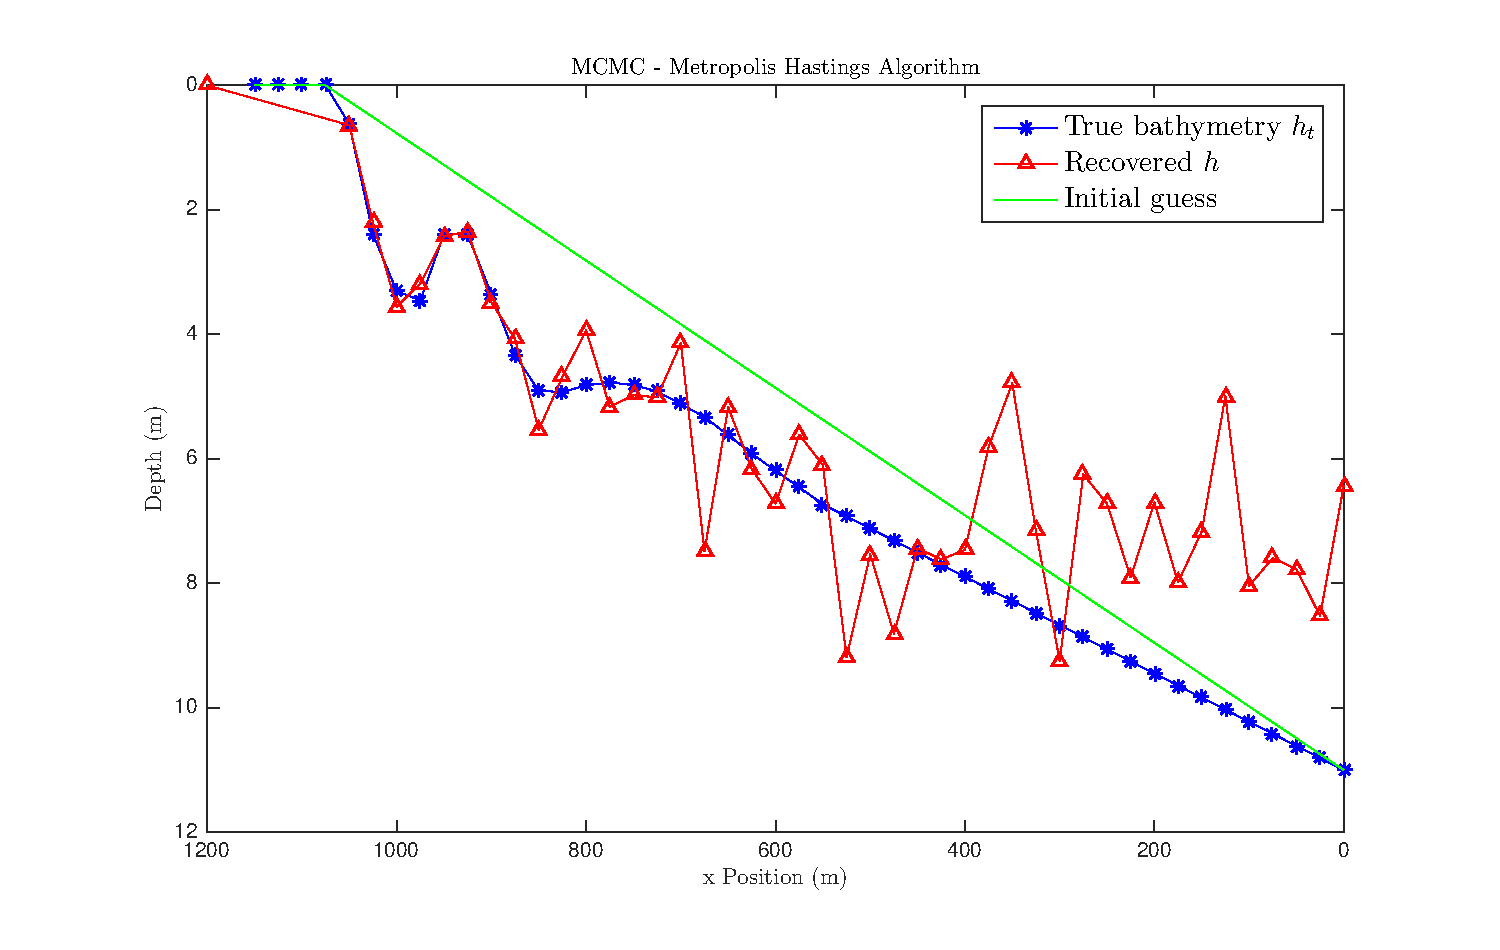
\includegraphics[scale=0.46]{img/MCMC-manufactured.eps} %plot20 
%\caption{Bathymetry estimate from the Bayesian Markov Chain Monte Carlo approach. The initial $h$ guess is shown in green, the true $h$ is shown in blue, and the derived estimate of $h$ is shown in red.}
%\label{mcmc-synthetic}
%\end{figure}
%
%Real $k$ data is then used to estimate the same bathymetry profile (Figure~\ref{mcmc-real}). We find...
%
%
%Unlike the other methods, the Bayesian approach results in a distribution of depth profiles which optimize $h$ given uncertain $k$. Measurements of wave number, $k$, are not perfect and our resulting distribution of depth profiles translates that uncertainty binto an ensemble of depth estimates which are consistent with the $k$ data to within uncertainty. Figures~\ref{mcmc-posterior-h-synthetic} and \ref{mcmc-posterior-h-real} show the resulting posterior depth distributions. Note that...
%



